\chapter{Anleitung zur GUI unter PyQt4}

\section{Allgemeiner Aufbau der GUI}

Starten des grgsm-scanner initiiert die GUI wie zu sehen in Abbildung:\ref{fig1}.
Das GUI-Fenster ist in zwei Felder aufgeteilt, ein kleineres Feld auf der linken Seite
und ein größeres auf der Rechten.
Im linken Feld werden die Kanäle dargestellt, welche nach und nach gescannt und hinzugefügt werden.
Im rechten Feld wird zu Beginn Informationen zur Projektarbeit ausgegeben. Diese wird durch die Informationen von ausgewählten Kanälen überschrieben, dazu jedoch später mehr.

\begin{figure}[H]
\centering
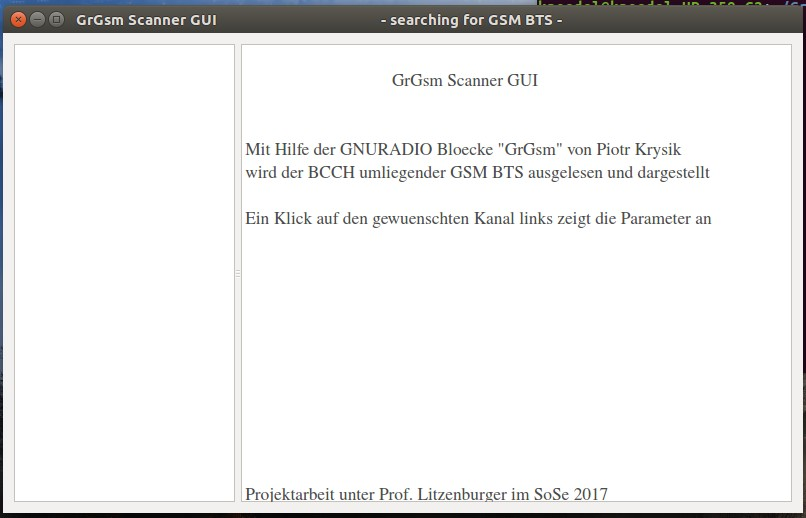
\includegraphics[scale=0.5]{GUI_Window}
\caption{Standard Fenster GUI}
\label{fig1}
\end{figure}

\noindent Solange die Suche nach Kanälen noch nicht abgeschlossen wurde, wird oben im Fensterrahmen \textbf{-searching for GSM BTS-} dargestellt (siehe Abbildung:\ref{fig1}).
Falls der Scan abgeschlossen ist, wird dies durch ein \textbf{Done} angezeigt, ersichtlich aus Bild \ref{fig2}. Außerdem sollten nun alle gefundenen Kanäle im linken Feld zu sehen sein.

\begin{figure}[H]
\centering
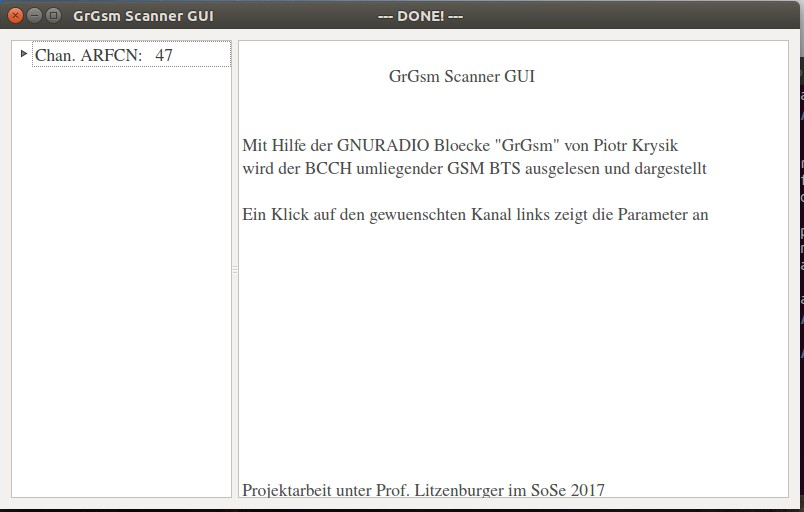
\includegraphics[scale=0.5]{GUI_Done}
\caption{abgeschlossener Scan}
\label{fig2}
\end{figure}

\noindent Falls Kanäle schon gescannt wurden und somit links auftauchen, können diese ausgewählt werden um Informationen der einzelnen Parameter einzusehen.
Unter den Parametern befinden sich der ARFCN, Frequenz, LAC, MCC, MNC, CID und die Power.
Zusätzlich werden ein paar weitere Informationen gegeben (siehe Abbildung:\ref{fig3}).
Sollte ein Maus angeschlossen sein können die Informationen auch durch eine Art Tooltip über mouse-hovering auf dem jeweiligen Kanal ausgegeben werden (siehe Abbildung:\ref{fig4}).

\begin{figure}[H]
\centering
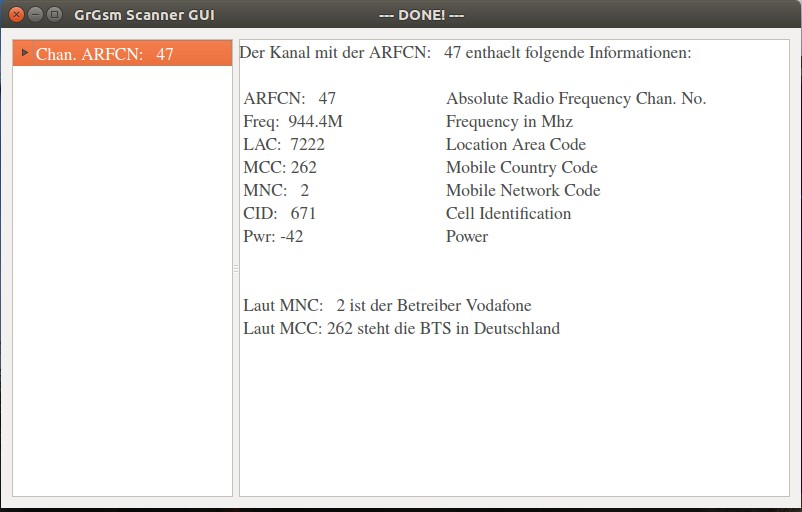
\includegraphics[scale=0.5]{GUI_Textinfo}
\caption{Info des BCCH}
\label{fig3}
\end{figure}

\begin{figure}[H]
\centering
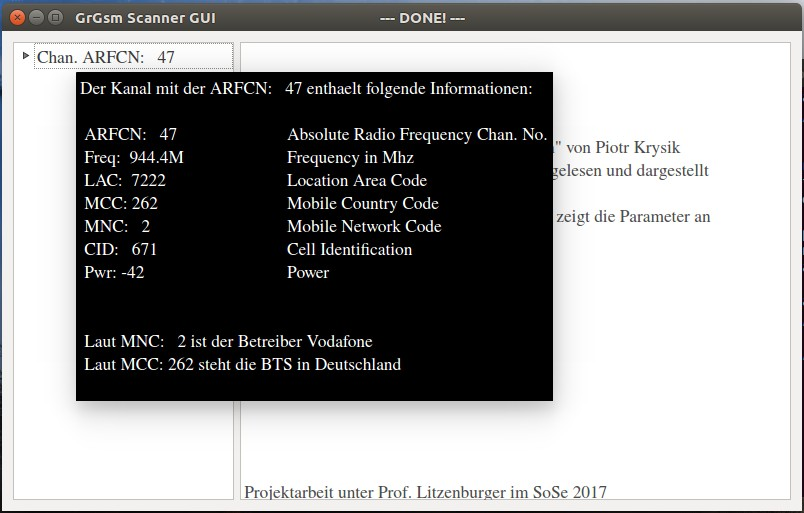
\includegraphics[scale=0.5]{GUI_Tooltip}
\caption{Mouseover Tooltip}
\label{fig4}
\end{figure}

\noindent Bei jedem Kanal ist es möglich durch einen kleinen Pfeil rechts daneben, diesen aufzurollen um die Parameter einzeln zu betrachten (siehe Abbildung:\ref{fig5}). Durch anklicken wieder auf die einzelnen Parameter wird die jeweilige Information dargestellt (siehe Abbildung:\ref{fig6}).


\begin{figure}[H]
\centering
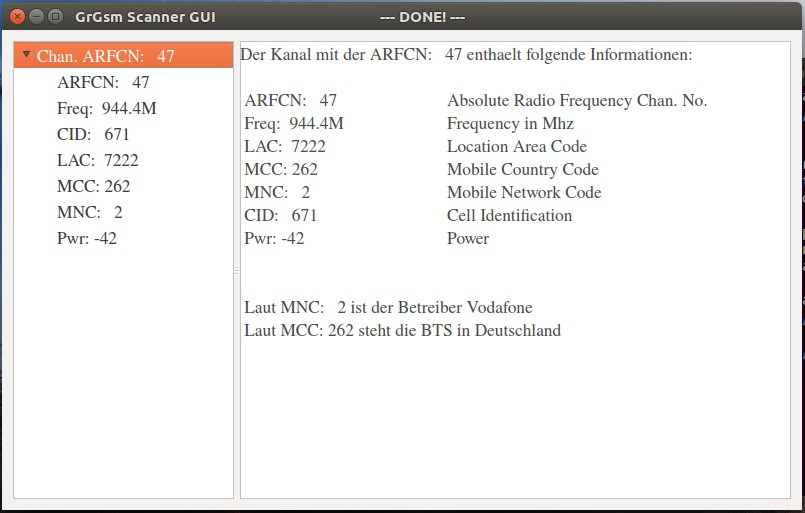
\includegraphics[scale=0.5]{GUI_aufgeklappt}
\caption{GUI Ansicht angeklickt}
\label{fig5}
\end{figure}

\begin{figure}[H]
\centering
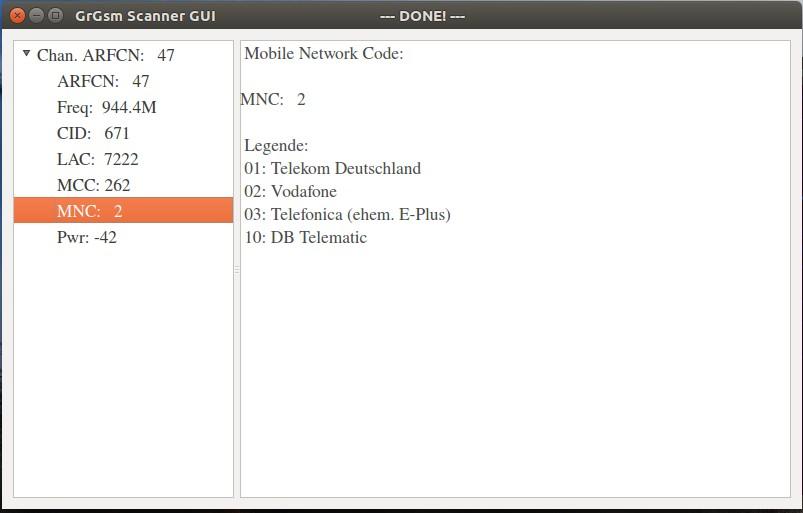
\includegraphics[scale=0.5]{GUI_childinfo}
\caption{Infos der Childnodes}
\label{fig6}
\end{figure}


\section{Anleitung zum Anpassen des textuellen Inhalts}

\subsection*{Anpassung der Titelseite}
Die Titelseite, wie im vorherigen Kapitel bereits erwähnt, welche zu sehen ist am Programmstart, kann durch Änderungen im folgenden Programmcode (Listing: \ref{code1}) angepasst werden.
Die Zeilenangaben links verdeutlichen zusätzlich, wo man dies im Programmcode finden kann.

\begin{code}[firstnumber=100,numbers=left,stepnumber=1, caption={Titelseite},captionpos=b,label={code1}]
self.text = QtGui.QLabel("\n"
                         " \t\t   GrGsm Scanner GUI\n\n\n"
                         " Mit Hilfe der GNURADIO Bloecke \"GrGsm\" von Piotr Krysik\n"
                         " wird der BCCH umliegender GSM BTS ausgelesen und dargestellt\n\n"
                         " Ein Klick auf den gewuenschten Kanal links zeigt die Parameter an\n\n\n\n\n\n\n\n\n\n\n"
                         " Projektarbeit unter Prof. Litzenburger im SoSe 2017\n"
                         " von Dennis Dette und Christian Kobiela\n\n"
                         , self.right)
\end{code} 

\subsection*{Anpassung der Parentnode}

Die Informationen, welche angezeigt werden wenn man einen gefunden Kanal anklickt, können in den folgenden Codezeilen geändert werden (Listing: \ref{code2}). Bisher werden wie zu sehen ist die einzelnen Parameter mit Werten dargestellt und Angaben über Land und Betreiber der BTS. 

\begin{code}[firstnumber=187,numbers=left,stepnumber=1, caption={Kanalinformation},captionpos=b,label={code2}]
parent_item.setToolTip(column,"Der Kanal mit der " + Buffer_Channel.ARFCN + 
		" enthaelt folgende Informationen: \n\n"
		+ " " +Buffer_Channel.ARFCN + " \t\tAbsolute Radio Frequency Chan. No.\n"
		+ " " +Buffer_Channel.FREQ + " \t\tFrequency in Mhz\n"
		+ " " +Buffer_Channel.LAC + " \t\tLocation Area Code\n"
		+ " " +Buffer_Channel.MCC + " \t\tMobile Country Code\n" 
		+ " " +Buffer_Channel.MNC + " \t\tMobile Network Code\n"
		+ " " +Buffer_Channel.CID + " \t\tCell Identification\n"			                        
		+ " " +Buffer_Channel.PWR+ " \t\tPower\n\n\n"
		+ " Laut " + Buffer_Channel.MNC + " ist der Betreiber " + Betreiber
		+ "\n Laut " + Buffer_Channel.MCC + " steht die BTS in " + str(Land)
		)
\end{code}

\subsection*{Anpassung der  Childnodes}

Nun zum letzten Teil, dessen Text angepasst werden kann, den Parameterinformationen. Diese sind einzusehen, wenn ein Kanal aufklappt ist. Hier werden durch auswählen der einzelnen Parameter die Informationen dargestellt, welche im Code \ref{code3} zu sehen sind. Die sieben Parameterinformationen werden in den verschiedenen If-Fällen definiert. 

\begin{code}[firstnumber=204,numbers=left,stepnumber=1,caption={Parameterinformationen},captionpos=b,label={code3}]
if k==0:
	item.setToolTip(column, " Absolute Radio Frequency Channel Number:\n\n " + Buffer_Channel.ARFCN 
	+ "\n\n In GSM cellular networks, an absolute radio-frequency channel number\n ""(ARFCN) is a code that specifies a pair of physical radio carriers used for\n ""transmission and reception in a land mobile radio system, one for the uplink\n ""signal and one for the downlink signal.\n\n "
	"ARFCN for GSM 900 \n "
	"ARFCN = (Chan. Freq - 45 Mhz- 890 Mhz)/200\n\n "
	"ARFCN for E GSM 900\n "
	"ARFCN = 1024 + (Chan. Freq - 45 Mhz - 890 Mhz)/200\n ")
elif k==1:
	item.setToolTip(column, " Frequency:\n\n " + Buffer_Channel.FREQ + "\n\n GSM Downlink Frequency")
elif k==2:
	item.setToolTip(column, " Cell Identification:\n\n " + Buffer_Channel.CID +
	"\n\n A GSM Cell ID (CID) is a generally unique number used\n "
	"to identify each base transceiver station (BTS) or\n "
	"sector of a BTS within a location area code (LAC) \n "
	"if not within a GSM network.")				
elif k==3:
	item.setToolTip(column, " Location Area Code:\n\n " + Buffer_Channel.LAC+
	"\n\n A location area is a set of base stations that are\n "
	"grouped together to optimise signalling.\n "
	"To each location area, a unique number called a location area code is assigned.\n ")
				    
					
elif k==4:
	item.setToolTip(column, " Mobile Country Code:\n\n " + Buffer_Channel.MCC +
	"\n\n The mobile country code consists of 3 decimal digits and the mobile\n "
	"network code consists of 2 or 3 decimal digits. The first \"2\" in 262\n "
	"stands for Europe, 62 for Germany")
				
elif k==5:
	item.setToolTip(column, " Mobile Network Code:\n\n" + Buffer_Channel.MNC +
	"\n\n Legende:\n 01: Telekom Deutschland\n 02: Vodafone\n 03: Telefonica (ehem. E-Plus)\n 10: DB Telematic")
	
elif k==6:
	item.setToolTip(column, " Power:\n\n " + Buffer_Channel.PWR + 
	"\n\n GSM needs at least a Power of -102dBm " )
\end{code}
 